% THIS IS SIGPROC-SP.TEX - VERSION 3.1
% WORKS WITH V3.2SP OF ACM_PROC_ARTICLE-SP.CLS
% APRIL 2009
%
% It is an example file showing how to use the 'acm_proc_article-sp.cls' V3.2SP
% LaTeX2e document class file for Conference Proceedings submissions.
% ----------------------------------------------------------------------------------------------------------------
% This .tex file (and associated .cls V3.2SP) *DOES NOT* produce:
%       1) The Permission Statement
%       2) The Conference (location) Info information
%       3) The Copyright Line with ACM data
%       4) Page numbering
% ---------------------------------------------------------------------------------------------------------------
% It is an example which *does* use the .bib file (from which the .bbl file
% is produced).
% REMEMBER HOWEVER: After having produced the .bbl file,
% and prior to final submission,
% you need to 'insert'  your .bbl file into your source .tex file so as to provide
% ONE 'self-contained' source file.
%
% Questions regarding SIGS should be sent to
% Adrienne Griscti ---> griscti@acm.org
%
% Questions/suggestions regarding the guidelines, .tex and .cls files, etc. to
% Gerald Murray ---> murray@hq.acm.org
%
% For tracking purposes - this is V3.1SP - APRIL 2009

\documentclass{acm_proc_article-sp}

\begin{document}

\title{Keystroke recovery using mobile phone accelerometers}

%
% You need the command \numberofauthors to handle the 'placement
% and alignment' of the authors beneath the title.
%
% For aesthetic reasons, we recommend 'three authors at a time'
% i.e. three 'name/affiliation blocks' be placed beneath the title.
%
% NOTE: You are NOT restricted in how many 'rows' of
% "name/affiliations" may appear. We just ask that you restrict
% the number of 'columns' to three.
%
% Because of the available 'opening page real-estate'
% we ask you to refrain from putting more than six authors
% (two rows with three columns) beneath the article title.
% More than six makes the first-page appear very cluttered indeed.
%
% Use the \alignauthor commands to handle the names
% and affiliations for an 'aesthetic maximum' of six authors.
% Add names, affiliations, addresses for
% the seventh etc. author(s) as the argument for the
% \additionalauthors command.
% These 'additional authors' will be output/set for you
% without further effort on your part as the last section in
% the body of your article BEFORE References or any Appendices.

\numberofauthors{4} %  in this sample file, there are a *total*
% of EIGHT authors. SIX appear on the 'first-page' (for formatting
% reasons) and the remaining two appear in the \additionalauthors section.
%
\author{
% You can go ahead and credit any number of authors here,
% e.g. one 'row of three' or two rows (consisting of one row of three
% and a second row of one, two or three).
%
% The command \alignauthor (no curly braces needed) should
% precede each author name, affiliation/snail-mail address and
% e-mail address. Additionally, tag each line of
% affiliation/address with \affaddr, and tag the
% e-mail address with \email.
%
% 1st. author
\alignauthor
Akshay Mittal\\
       \affaddr{Princeton University}\\
% 2nd. author
\alignauthor Wathsala Vithanage\\
       \affaddr{Princeton University}\\
% 3rd. author
\alignauthor Stephen Lin\\
       \affaddr{Princeton University}\\
\and  % use '\and' if you need 'another row' of author names
% 4th. author
\alignauthor Jennifer Guo\\
       \affaddr{Princeton University}\\
}

\maketitle
\begin{abstract}
[to - fill]
\end{abstract}

\section{Introduction}
\label{sec:introduction}
\noindent Mobile phones~\cite{spiphone} are becoming increasingly powerful
devices. In addition to being able to run applications ranging from email
clients to web browsers, a progressively sophisticated set of sensors are
enabling these devices to more actively interface with the world
around them. From gestures captured by accelerometers for games
to augmented reality applications displaying metadata tags on video
from the camera in real-time, mobile phones are becoming adept
at capturing and harnessing rich features and data from their surroundings.

Unfortunately, the array of sensors in these devices can also be
used in unintended ways. As many have suggested, malware could
potentially gain access to a mobile phone's camera to take photos or
video of the owner and their surroundings~\cite{cheng2007mobile}. In cases where
the camera may not be pointed at an interesting target, a malicious
application could instead attempt to activate the device's microphone
and record ambient sounds or syphon GPS data to track the
target's location
\cite{dagon2004mobile, cai2009defending, enck2010taintdroid, egele2011pios}.
Recognizing the potential for the leakage of sensitive information, many
modern mobile phone operating systems provide mechanisms by which access to
such sensors is protected by explicit permission from the user. For instance,
the manifest files included with every Android application provide an
unambiguous list of all of permissions an application may ever request
at installation time. Should an application not request access
to these resources or the user deny the application such rights, the
application will not be able to potentially abuse these resources.
However, access to all of the sensors contained in these devices are
not so tightly controlled.

In this paper, we demonstrate that unfettered access to the
accelerometers available on many mobile phones can allow for significant
unintended leakage of information from a user's environment.
We show that a malicious application with access to the accelerometer
feed can record and reconstruct the keypresses made
on a nearby keyboard based solely on the observed vibrations. We
develop profiles for keypress events using boosted Random Forests,
which creates an abstract representation of the relationship between
the keystroke signal and the alphabet typed. We then recover the typed content
by translating from our intermediary form to English words using a number
of different dictionaries. Such tasks are not a trivial application of
standard techniques, especially when compared to previous efforts
in this space. Specifically, we must overcome much lower sensor
sampling rates than has been experienced in the related acoustic
and electromagnetic-based eavesdropping attacks, which makes
deciphering individual keypresses extremely difficult.

Through this, we make the following contributions in this paper:
\begin{enumerate}
\item {\bf Develop an infrastructure for characterizing keypress vibrations}: We
capture, analyze and develop profiles of keypress events on a nearby
keyboard based on the vibrations created when they are pressed. Our inputs are
then processed using a set boosted Random Forests to create an intermediary
representation, which is combined with candidate dictionaries
to successfully recover words at rates as high as \_\_ %.
\item {\bf Dataset made publicly available}: To the best of our knowledge,
there does not exists a dataset with
the keystrokes for the vibrations recorded using an accelerometer. In this
paper, we demonstrate we construct the dataset of keystroke vibrations,
recorded using the accelerometer, present in a smartphone and make
the dataset publicly available to enhance further research on this topic. Given
the widespread about security breaches and email leaks, we perceive this to be
of great importance in motivating the mobile operating system manufacturers
to restrict the usage of accelerometers to permitted applications only.\\
\end{enumerate}
\noindent Note that our approach is greatly influenced by the work of
Marquardt \emph{et. al}~\cite{spiphone} and we present key differences with our
approach.

\section{Related Work}
Researchers have studied malicious code on mobile devices that
learn information about the device owner using other embedded sensors.
In the most closely related work to our paper, Marquardt \emph{et. al}
\cite{spiphone} propose \emph{(sp)iPhone} which uses motion sensors in the
iPhone 4
to infer keystrokes of nearby laptop users. \emph{(sp)iPhone} uses 3 labels for
each pair of keystrokes in order to determine the correct identification for
the letters of the word. The location of the key is modelled using a neural
network trained on 150 keystrokes for each letter of the English alphabet.
A profile is then constructed for each pair using the neural network and
determines and models the distance between the two events. The predictions
of the neural network are matched against a dictionary to determine the top
matches. The accuracy achieved is roughly 80\% but this decreases to 40\%
as the size of the dictionary increases.

In a very similar, but orthogonal, use case, Owusu \emph{et. al}
\cite{owusu2012accessory}
present the threat of applications which extract the keystrokes of the
user's typing on the smartphone screen itself. Again, due to no restrictions
on the usage of the accelerometer, they are able to extract 6-character
passwords in as few as 4.5 trials(median). TouchLogger~\cite{cai2011touchlogger}
uses orientation of the smartphone device to infer the keystrokes.

\section{Threat Model}

Our attack is based upon two observations:

Many users like to place their smartphone close to their laptop while working, so that it is easily accessible and notifications are not missed.

Furthermore we note that while smartphones offer a broad range of sensers such as microphone, GPS, gyroscope and accelerometer, the accelerometer is the only sensor to which access is not protected in any current mobile phone operating system.

\section{Framework Description}

\subsection{Dataset Capturing}

\begin{figure}
\centering
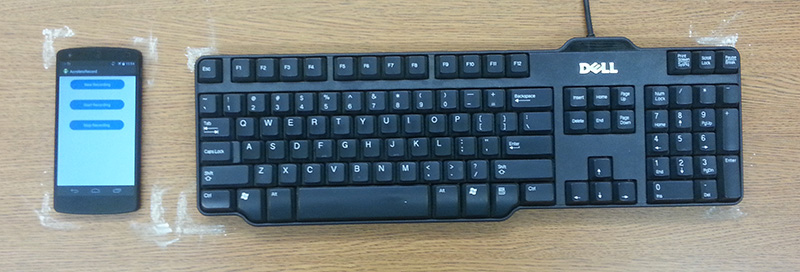
\includegraphics[width=0.5\textwidth]{img/setup}
\caption{Threat model of a smartphone placed next to a keyboard. Used in our experimental setup to capture the dataset.
}
\label{fig:setup}
\end{figure}

Our experimental setup is shown in fig.\ref{fig:setup}. We placed a Dell USB keyboard and a LG Nexus smartphone on a wooden table. No other items were placed on or were touching the table. All keys were pressed with the index finger of the right hand. The hands do not touch the keyboard or table, and the fingers do not pause on the keyboard but only touch it during the brief duration of the key press.

We recorded 1000 datapoints in 40 sessions with 25 letters in each sessions. For each session we generate a sequence of 25 random letters and display the letters in 3 second intervals to ensure an even recording of the letters and to ensure that there is no bias towards a specific letter. For the data capturing we developed an Android app that reads from the hardware accelerometer and syncs with our laptops, where we further process the data. The raw accelerometer data as returned by Android contains the $x$, $y$ and $z$-direction components of the acceleration of the vibration received. We calculate the G-force magnitude as $\sqrt{x^2+y^2+z^2}-g$ where $g = 9.81$ is the acceleration due to gravity.

\begin{figure}
\centering
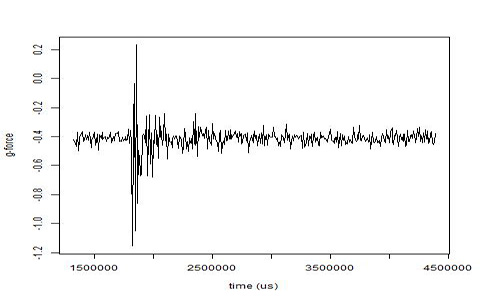
\includegraphics[width=0.5\textwidth]{img/signal2}
\caption{Sample Recording for letter 'a'}
\label{fig:signal}
\end{figure}

The original recording will contain a large spike at the beginning and end due to the pressing of "Start" and "Stop" on the recording app. We cut off these noise signals and further segment the data into 25 individual data points. An example of a plot of one such signal is shown in fig.\ref{fig:signal}.


\section{Implementation}

\section{Experimental Results}


\section{Conclusions}

\subsection{Future Work}

Mobile browsers having allowing access to accelerometer data,

http://blogs.adobe.com/cantrell/archives/2012/03/accessing-the-accelerometer-and-gyroscope-in-javascript.html

http://isthisanearthquake.com/

http://isthisanearthquake.com/seismograph.html

%ACKNOWLEDGMENTS are optional
\section{Acknowledgments}


%
% The following two commands are all you need in the
% initial runs of your .tex file to
% produce the bibliography for the citations in your paper.
\bibliographystyle{unsrt}
\bibliography{sigproc}  % sigproc.bib is the name of the Bibliography in this case
% You must have a proper ".bib" file
%  and remember to run:
% latex bibtex latex latex
% to resolve all references
%
% ACM needs 'a single self-contained file'!
%
%APPENDICES are optional
%\balancecolumns
\appendix
%Appendix A

\section{Appendix Section}

\subsection{Appendix Subsection}

\balancecolumns
% That's all folks!
\end{document}
